\documentclass[journal]{IEEEtran}

% --- Core Packages ---
\usepackage{_internals/preamble} % Load all common packages from preamble.sty

% --- Bibliography Setup (BibLaTeX) ---
% Load biblatex *after* the class and preamble, but *before* \begin{document}
\usepackage[backend=biber,style=ieee,natbib=true, maxnames=6, minnames=1, date=year, doi=false, isbn=false, url=false]{biblatex} % Using biblatex-ieee
% Options explained:
% maxnames=6: Show up to 6 authors, then use 'et al.'
% minnames=1: Use 'et al.' if there's more than 1 author *and* maxnames is exceeded.
% date=year: Only show year, not month/day
% doi=false, isbn=false, url=false: Hide these fields by default (common for IEEE)
\addbibresource{../pustaka.bib} % Path to your master .bib file

% journal_ui_ana/indonesia/commands.tex
% Diadaptasi dari settings.tex dan journal_ieee/commands.tex

% --- Informasi Dokumen dari settings.tex (Skripsi) ---
\newcommand{\myJudulIndonesia}{Implementasi dan Analisis Efektivitas Vxlang \textit{Code Virtualization} dalam mempersulit \textit{Reverse Engineering}}
\newcommand{\myPenulis}{Seno Pamungkas Rahman}
\newcommand{\myNPM}{2106731586} % Mungkin tidak diperlukan untuk jurnal, tapi disimpan
\newcommand{\myPembimbing}{Dr. Ruki Harwahyu, S.T., M.T., M.Sc.} % Sesuai contoh PDF Anda (dengan gelar)
\newcommand{\myDepartment}{Departemen Teknik Elektro}
\newcommand{\myFaculty}{Fakultas Teknik}
\newcommand{\myUniversity}{Universitas Indonesia}
\newcommand{\myAddress}{Kampus UI Depok 16424, Jawa Barat, Indonesia}
\newcommand{\myEmail}{seno.pamungkas@ui.ac.id}

\newcommand{\myTitleEnglish}{Implementation and Analysis of the Effectiveness of Vxlang Code Virtualization in Complicating Reverse Engineering} % Dari settings.tex \judulInggris, sedikit disesuaikan kapitalisasinya agar umum untuk judul

\newcommand*{\Assets}{../../assets/pics}%

\renewcommand{\figurename}{\bo{Figure}}
%
%
\renewcommand{\tablename}{\bo{Table}}
%
%
\newcommand{\pic}{Figure}
%
%
\newcommand{\tab}{Table}
%
%
\newcommand{\equ}{Equation}


% --- Start of Document ---
\begin{document}

% --- Paper Title ---
\title{\journalTitle}

% --- Author Information ---
\author{\IEEEauthorblockN{\authorOne\IEEEauthorrefmark{1}} % Use refmark if needed for affiliations/notes
        % , \IEEEauthorblockN{Author Two Name\IEEEauthorrefmark{2}} % Add other authors
\IEEEauthorblockA{\textit{\authorOneAffiliation} \\ Email: \authorOneEmail}
% \IEEEauthorblockA{\IEEEauthorrefmark{2}\textit{Affiliation Author Two}} % Corresponding affiliation
% --- Add more authors/affiliations as needed ---

\thanks{Manuscript received Month DD, YYYY; revised Month DD, YYYY. This work was supported in part by [Funding Agency, Grant Number, if any]. (Corresponding author: \correspondingAuthor.)} % Update or remove as appropriate
% \thanks{\authorOne is with the Department of Electrical Engineering, Faculty of Engineering, Universitas Indonesia, Depok, 16424 Indonesia (e-mail: \authorOneEmail).} % Standard IEEE affiliation format
% \thanks{Author Two is with ...} % Add other author affiliations if needed
}

% --- Paper Headers ---
% Optional: Customize headers for published version/preprint
% \markboth{IEEE Transactions on Dependable and Secure Computing,~Vol.~XX, No.~XX, Month~YYYY}%
% {Rahman: Analysis of VxLang Code Virtualization Effectiveness}

% --- Make Title Area ---
\maketitle

% --- Abstract and Keywords ---
\begin{abstract}
Reverse engineering poses a significant threat to software security, enabling attackers to analyze, understand, and illicitly modify program code. Code obfuscation techniques, particularly code virtualization, offer a promising defense mechanism. This paper presents an implementation and analysis of the effectiveness of code virtualization using the VxLang framework in enhancing software security against reverse engineering. We applied VxLang's virtualization to critical sections of case study applications, including authentication logic. Static analysis using Ghidra and dynamic analysis using x64dbg were performed on both the original and virtualized binaries. The results demonstrate that VxLang significantly increases the complexity of reverse engineering. Static analysis tools struggled to disassemble and interpret the virtualized code, failing to identify instructions, functions, or meaningful data structures. Dynamic analysis was similarly hampered, with obfuscated control flow and the virtual machine's execution model obscuring runtime behavior and hindering debugging attempts. However, this enhanced security comes at the cost of substantial performance overhead, observed in QuickSort algorithm execution and AES encryption benchmarks, along with a significant increase in executable file size. The findings confirm that VxLang provides robust protection against reverse engineering but necessitates careful consideration of the performance trade-offs for practical deployment.
\end{abstract}

\begin{IEEEkeywords}
Code Obfuscation, Code Virtualization, Software Protection, Reverse Engineering, VxLang, Security Analysis, Performance Overhead.
\end{IEEEkeywords}


% --- Main Content ---
\IEEEpeerreviewmaketitle % Command for peer review markers

\section{Introduction}
% The very first letter is a 2 line initial drop letter followed
% by the rest of the first word in caps.
% 
% form to use if the first word consists of a single letter:
% \IEEEPARstart{A}{demo} file is ....
% 
% form to use if you need the single drop letter followed by
% normal text (unknown if ever used by the IEEE):
% \IEEEPARstart{A}{}demo file is ....
% 
% Some journals put the first two words in caps:
% \IEEEPARstart{T}{his demo} file is ....
% 
% Here we have the typical use of a "T" for an initial drop letter
% and "HIS" in caps to complete the first word.
\IEEEPARstart{T}{his} demo file is intended to serve as a ``starter file''
for IEEE journal papers produced under \LaTeX\ using
IEEEtran.cls version 1.8b and later.
% You must have at least 2 lines in the paragraph with the drop letter
% (should never be an issue)
I wish you the best of success.

\hfill mds
 
\hfill August 26, 2015

\subsection{Subsection Heading Here}
Subsection text here.

% needed in second column of first page if using \IEEEpubid
%\IEEEpubidadjcol

\subsubsection{Subsubsection Heading Here}
Subsubsection text here.


% An example of a floating figure using the graphicx package.
% Note that \label must occur AFTER (or within) \caption.
% For figures, \caption should occur after the \includegraphics.
% Note that IEEEtran v1.7 and later has special internal code that
% is designed to preserve the operation of \label within \caption
% even when the captionsoff option is in effect. However, because
% of issues like this, it may be the safest practice to put all your
% \label just after \caption rather than within \caption{}.
%
% Reminder: the "draftcls" or "draftclsnofoot", not "draft", class
% option should be used if it is desired that the figures are to be
% displayed while in draft mode.
%
%\begin{figure}[!t]
%\centering
%\includegraphics[width=2.5in]{myfigure}
% where an .eps filename suffix will be assumed under latex, 
% and a .pdf suffix will be assumed for pdflatex; or what has been declared
% via \DeclareGraphicsExtensions.
%\caption{Simulation results for the network.}
%\label{fig_sim}
%\end{figure}

% Note that the IEEE typically puts floats only at the top, even when this
% results in a large percentage of a column being occupied by floats.


% An example of a double column floating figure using two subfigures.
% (The subfig.sty package must be loaded for this to work.)
% The subfigure \label commands are set within each subfloat command,
% and the \label for the overall figure must come after \caption.
% \hfil is used as a separator to get equal spacing.
% Watch out that the combined width of all the subfigures on a 
% line do not exceed the text width or a line break will occur.
%
%\begin{figure*}[!t]
%\centering
%\subfloat[Case I]{\includegraphics[width=2.5in]{box}%
%\label{fig_first_case}}
%\hfil
%\subfloat[Case II]{\includegraphics[width=2.5in]{box}%
%\label{fig_second_case}}
%\caption{Simulation results for the network.}
%\label{fig_sim}
%\end{figure*}
%
% Note that often IEEE papers with subfigures do not employ subfigure
% captions (using the optional argument to \subfloat[]), but instead will
% reference/describe all of them (a), (b), etc., within the main caption.
% Be aware that for subfig.sty to generate the (a), (b), etc., subfigure
% labels, the optional argument to \subfloat must be present. If a
% subcaption is not desired, just leave its contents blank,
% e.g., \subfloat[].


% An example of a floating table. Note that, for IEEE style tables, the
% \caption command should come BEFORE the table and, given that table
% captions serve much like titles, are usually capitalized except for words
% such as a, an, and, as, at, but, by, for, in, nor, of, on, or, the, to
% and up, which are usually not capitalized unless they are the first or
% last word of the caption. Table text will default to \footnotesize as
% the IEEE normally uses this smaller font for tables.
% The \label must come after \caption as always.
%
%\begin{table}[!t]
%% increase table row spacing, adjust to taste
%\renewcommand{\arraystretch}{1.3}
% if using array.sty, it might be a good idea to tweak the value of
% \extrarowheight as needed to properly center the text within the cells
%\caption{An Example of a Table}
%\label{table_example}
%\centering
%% Some packages, such as MDW tools, offer better commands for making tables
%% than the plain LaTeX2e tabular which is used here.
%\begin{tabular}{|c||c|}
%\hline
%One & Two\\
%\hline
%Three & Four\\
%\hline
%\end{tabular}
%\end{table}


% Note that the IEEE does not put floats in the very first column
% - or typically anywhere on the first page for that matter. Also,
% in-text middle ("here") positioning is typically not used, but it
% is allowed and encouraged for Computer Society conferences (but
% not Computer Society journals). Most IEEE journals/conferences use
% top floats exclusively. 
% Note that, LaTeX2e, unlike IEEE journals/conferences, places
% footnotes above bottom floats. This can be corrected via the
% \fnbelowfloat command of the stfloats package.

\section{Related Work} \label{sec:related_work}
Protecting software from unauthorized analysis and tampering is a long-standing challenge. Reverse engineering techniques are constantly evolving, necessitating more sophisticated protection mechanisms. This section reviews relevant work in code obfuscation, focusing on code virtualization.

\subsection{Code Obfuscation Techniques}
Obfuscation aims to increase the complexity of understanding code without altering its functionality \cite{Jin24}. Techniques operate at different levels:

\subsubsection{Source Code Obfuscation} Modifies the human-readable source code.
\begin{itemize}
    \item \textbf{Layout Obfuscation:} Alters code appearance (e.g., scrambling identifiers \cite{Cha04}, removing comments/whitespace \cite{Bal11}). Provides minimal security against automated tools.
    \item \textbf{Data Obfuscation:} Hides data representation (e.g., encoding strings \cite{Ert05, Fuk08, Kov13}, splitting/merging arrays, using equivalent but complex data types). Can make data analysis harder. Techniques like instruction substitution \cite{LeD12, Dar10} and mixed boolean-arithmetic \cite{Liu21, Sch22, Zho07} fall under this category, obscuring data manipulation logic.
    \item \textbf{Control Flow Obfuscation:} Modifies the program's execution path logic. Examples include inserting bogus control flow \cite{LiY211}, using opaque predicates (conditional statements whose outcome is known at obfuscation time but hard to determine statically \cite{XuD16}), and control flow flattening, which transforms structured code into a large switch statement, obscuring the original logic \cite{Lás09}.
\end{itemize}

\subsubsection{Bytecode Obfuscation} Targets intermediate code (e.g., Java bytecode, .NET CIL, LLVM IR). Techniques include renaming identifiers, control flow obfuscation, string encryption, and inserting dummy code \cite{Pie18, Yak20}. Effective against decompilation back to high-level source code.

\subsubsection{Binary Code Obfuscation} Operates on the final machine-executable code.
\begin{itemize}
    \item \textbf{Code Packing/Encryption:} Compresses or encrypts the original code, requiring a runtime stub to unpack/decrypt it before execution \cite{Rou13}. Primarily hinders static analysis but reveals the original code in memory during execution.
    \item \textbf{Control Flow Manipulation:} Uses indirect jumps/calls, modifies call/ret instructions, or chunks code into small blocks with jumps to disrupt linear disassembly and analysis \cite{Rou13}.
    \item \textbf{Constant Obfuscation:} Hides constant values through arithmetic/logical operations \cite{Rou13}.
    \item \textbf{Code Virtualization:} As discussed below, this is considered one of the strongest binary obfuscation techniques.
\end{itemize}

\subsection{Code Virtualization (VM-Based Obfuscation)}
Code virtualization translates native code into a custom bytecode format, executed by an embedded virtual machine (VM) \cite{Ore06, Zho24}. This creates a significant barrier for reverse engineers, as standard tools cannot interpret the custom ISA \cite{Sal18}. The attacker must first understand the VM's architecture, handler implementations, and bytecode mapping, which is a complex and time-consuming task \cite{Don20, Hac24}.

Key aspects of VM-based obfuscation include:
\begin{itemize}
    \item \textbf{Custom ISA:} Each protected application can potentially have a unique or mutated set of virtual instructions, hindering signature-based detection or analysis reuse. Oreans highlights the possibility of generating diverse VMs for different protected copies \cite{Ore06}.
    \item \textbf{VM Architecture:} Typical VM components include fetch, decode, dispatch, and handler units, mimicking CPU operations but implemented in software \cite{Sal18, Hac24}. The complexity and implementation details of these handlers directly impact both security and performance.
    \item \textbf{Security vs. Performance Trade-off:} The interpretation layer introduced by the VM inherently adds performance overhead compared to native execution. The level of obfuscation within the VM handlers and the complexity of the virtual instructions influence this trade-off.
\end{itemize}

Several commercial tools like VMProtect \cite{VMP24} and Themida \cite{Ore24} (which also includes virtualization features beyond basic packing) employ code virtualization. Academic research has also explored techniques like symbolic deobfuscation to analyze virtualized code \cite{Sal18} and methods to enhance virtualization robustness, such as virtual code folding \cite{Don20}.

\subsection{VxLang in Context}
VxLang positions itself as a comprehensive framework offering binary protection, code obfuscation (including flattening), and code virtualization \cite{VxLang}. Its approach involves transforming native x86-64 code into an internal bytecode executed by its VM. This study aims to provide an empirical evaluation of the effectiveness of VxLang's virtualization component against standard reverse engineering practices and quantify its associated performance costs, contributing practical insights into its utility as a software protection mechanism. Unlike analyzing established commercial protectors, this work focuses on the specific implementation and impact of the VxLang framework.

\section{Methodology} \label{sec:methodology}
This research employs an experimental approach to evaluate the effectiveness of VxLang's code virtualization. We compare the reverse engineering difficulty and performance characteristics of software binaries before and after applying VxLang's virtualization.

\subsection{Experimental Design}
A comparative study design was used, involving a control group (original, non-virtualized binaries) and an experimental group (binaries with critical sections virtualized by VxLang).

\begin{itemize}
    \item \textbf{Independent Variable:} Application of VxLang code virtualization (Applied vs. Not Applied).
    \item \textbf{Dependent Variables:}
        \begin{itemize}
            \item \textit{Reverse Engineering Difficulty:} Qualitatively assessed based on the effort required for static analysis (code understanding, logic identification, patching attempts using Ghidra) and dynamic analysis (runtime tracing, memory inspection, manipulation attempts using x64dbg). Success/failure of bypassing authentication logic was recorded.
            \item \textit{Performance Overhead:} Quantitatively measured via execution time for specific computational tasks (QuickSort, AES encryption/decryption).
            \item \textit{File Size Overhead:} Quantitatively measured by comparing the size (in bytes) of the final executable files.
        \end{itemize}
\end{itemize}

\subsection{Study Objects}
Two categories of applications were developed and analyzed:

\subsubsection{Authentication Case Study Applications} Simple applications simulating user login were created to serve as targets for reverse engineering analysis focused on bypassing the authentication mechanism. Variants included:
    \begin{itemize}
        \item \textbf{Interface Types:} Console (CLI), Qt Widgets (GUI), Dear ImGui (Immediate Mode GUI).
        \item \textbf{Authentication Mechanisms:} Hardcoded credentials (comparing input against string literals) and Cloud-based validation (sending credentials via HTTP POST to a local backend server).
    \end{itemize}
    For each variant, the core authentication logic (comparison function or the call to the cloud request function and subsequent result check) was targeted for virtualization in the experimental group.

\subsubsection{Performance Benchmark Applications} Applications designed to measure the performance impact of virtualization on specific computational tasks:
    \begin{itemize}
        \item \textbf{QuickSort Benchmark:} Implemented a standard recursive QuickSort algorithm. The core recursive function was virtualized. Tested with varying array sizes (100 to 1,000,000 elements).
        \item \textbf{AES Encryption Benchmark:} Implemented AES-256-CBC encryption/decryption using OpenSSL's EVP API. The loop performing batch encryption/decryption operations on 1GB of data was virtualized.
        \item \textbf{File Size Benchmark:} A minimal application with embedded dummy data to assess the baseline size increase due to the inclusion of the VxLang runtime.
    \end{itemize}

\subsection{Instrumentation and Materials}
\begin{itemize}
    \item \textbf{Hardware:} Standard Windows 11 (64-bit) PC.
    \item \textbf{Development Tools:} Clang/clang-cl (C++17), CMake, Ninja, Neovim.
    \item \textbf{Libraries/Frameworks:} VxLang SDK, Qt 6, Dear ImGui (+GLFW/OpenGL3 backend), OpenSSL 3.x, libcurl, nlohmann/json.
    \item \textbf{Analysis Tools:} Ghidra (v11.x) for static analysis, x64dbg (latest snapshot) for dynamic analysis.
    \item \textbf{Performance Measurement:} C++ \texttt{std::chrono::high\_resolution\_clock} for timing, \texttt{std::filesystem::file\_size} for file size.
\end{itemize}

\subsection{Data Collection Procedure}

\subsubsection{Security Analysis}
For each authentication application (original and virtualized):
    \begin{enumerate}
        \item \textbf{Static Analysis (Ghidra):} Load executable, search for relevant strings (e.g., "Failed", "Authorized", potential credentials), analyze disassembly/decompilation around string references or entry points, identify conditional jumps controlling authentication success/failure, attempt static patching to bypass logic. Record qualitative observations on difficulty.
        \item \textbf{Dynamic Analysis (x64dbg):} Run executable under debugger, search for strings/patterns at runtime, set breakpoints at suspected logic locations (identified via static analysis or runtime observation), step through execution, observe register/memory values, attempt runtime manipulation (patching conditional jumps, altering flags/memory) to bypass authentication. Record qualitative observations and success/failure of bypass attempts.
    \end{enumerate}

\subsubsection{Performance Analysis}
For each benchmark application (original and virtualized):
    \begin{enumerate}
        \item \textbf{Execution Time:} Run QuickSort benchmark 100 times per data size, record individual times. Run AES benchmark on 1GB data, record total encryption/decryption time. Use \texttt{std::chrono}. Calculate average, standard deviation (for QuickSort), and throughput (for AES).
        \item \textbf{File Size:} Measure the size of the final executable file in bytes using \texttt{std::filesystem::file\_size}.
    \end{enumerate}

\subsection{Data Analysis Techniques}
\begin{itemize}
    \item \textbf{Qualitative Security Data:} Descriptive analysis based on observation notes comparing the reverse engineering effort and success rates between control and experimental groups for both static and dynamic analysis phases.
    \item \textbf{Quantitative Performance Data:} Calculation of descriptive statistics (mean, standard deviation), percentage overhead for execution time, throughput calculation (MB/s), and percentage increase in file size. Comparative tables and graphs will be used for presentation.
    \item \textbf{Trade-off Analysis:} Synthesis of security findings and performance results to evaluate the balance between protection enhancement and performance/size costs introduced by VxLang.
\end{itemize}

\section{Implementation Details} \label{sec:implementation}
This section briefly outlines the key aspects of the experimental setup and the integration of VxLang.

\subsection{Development Environment}
All development and testing were conducted on a Windows 11 (64-bit) system. The Clang compiler (v19.1.3, via \texttt{clang-cl} for MSVC ABI compatibility) targeting x86-64 was used with the C++17 standard. CMake (v3.31) and Ninja (v1.12.1) managed the build process. Essential libraries included the VxLang SDK, Qt 6, Dear ImGui, OpenSSL 3.x, and libcurl, linked appropriately via CMake.

\subsection{VxLang Integration}
VxLang was applied to the target applications using its Software Development Kit (SDK) and external processing tool.

\subsubsection{Code Marking} Critical code sections intended for virtualization were demarcated in the C++ source code using the SDK's macros, primarily \texttt{VL\_VIRTUALIZATION\_BEGIN} and \texttt{VL\_VIRTUALIZATION\_END}. For instance, in the authentication logic:

\begin{minted}[fontsize=\small, breaklines, escapeinside=||]{cpp}
// ... Input username/password ...
#ifdef USE_VL_MACRO
VL_VIRTUALIZATION_BEGIN; // Mark start
#endif

if (check_credentials(username, password)) {
    // Authorized path
} else {
    // Unauthorized path
}

#ifdef USE_VL_MACRO
VL_VIRTUALIZATION_END; // Mark end
#endif
// ...
\end{minted}
Similar macros were placed around the recursive \texttt{quickSort} function body and the main encryption/decryption loop in the AES benchmark.

\subsubsection{Build Process} The CMake configuration was set up to generate two distinct build types:
\begin{enumerate}
    \item \textbf{Original Build:} Compiled without the \texttt{USE\_VL\_MACRO} preprocessor definition and without linking the VxLang library. Produces the baseline executable (e.g., \texttt{app\_qt.exe}).
    \item \textbf{Intermediate Build (VM Marked):} Compiled with \texttt{USE\_VL\_MACRO} defined and linked against \texttt{vxlib64.lib}. Produces an intermediate executable containing the VxLang markers (e.g., \texttt{app\_qt\_vm.exe}).
\end{enumerate}

\subsubsection{Virtualization Processing}
The intermediate executables (e.g., \texttt{app\_qt\_vm.exe}) generated by the build process, which contain the VxLang markers and are linked against the VxLang library, were then directly processed using the VxLang command-line tool. This was done by executing the tool with the intermediate executable as an argument, for example:

\begin{minted}[fontsize=\small, breaklines, escapeinside=||, frame=none, bgcolor=lightgray!20]{bash}
vxlang.exe app_qt_vm.exe
\end{minted}

This command automatically processes the input file, replacing the native code within the marked sections (\texttt{VL\_VIRTUALIZATION\_BEGIN/END}) with its corresponding virtualized bytecode and embedding the necessary VM runtime. The tool generates the final virtualized executable in the same directory, automatically appending \texttt{\_vxm} to the original filename (e.g., producing \texttt{app\_qt\_vxm.exe}). This resulting \texttt{*\_vxm.exe} file was then used for all subsequent testing and analysis. No explicit configuration files (like JSON) were used in this processing step.

\subsection{Lilith RAT Preparation}
The Lilith RAT client source code \cite{LilithRAT} was compiled using the same environment (Clang/clang-cl, CMake, Ninja). For the virtualized version, VxLang SDK macros (\texttt{VL\_VIRTUALIZATION\_BEGIN/END}) were strategically placed around key functional blocks within the client's source code, targeting areas responsible for connection handling, command processing, and core RAT functionalities. An intermediate executable (\texttt{Lilith\_Client\_vm.exe}) was built with the \texttt{USE\_VL\_MACRO} flag and linked against \texttt{vxlib64.lib}. This intermediate file was then directly processed using the external VxLang command-line tool (\texttt{vxlang.exe Lilith\_Client\_vm.exe}) to produce the final virtualized Lilith client executable (\texttt{Lilith\_Client\_vxm.exe}) used in the analysis. The Lilith server component remained unmodified.

It is pertinent to note that the strategic placement of VxLang macros was crucial for maintaining the functional integrity of the Lilith RAT client. Initial attempts to virtualize larger, more complex code blocks, particularly those involving intricate control flow (e.g., entire switch-case statements handling packet types) or direct network I/O calls, occasionally resulted in application instability or crashes. Stable functionality was achieved by applying virtualization more granularly to specific, well-contained functions or critical logical segments, underscoring the need for careful, iterative testing when integrating VM-based obfuscation into complex applications.

\section{Results and Discussion} \label{sec:results_discussion}
This section presents the results of the security analysis and performance measurements, followed by a discussion of the findings.

\subsection{Security Analysis Results}
The effectiveness of VxLang virtualization was evaluated through static and dynamic analysis attempts to understand and bypass the authentication logic in the case study applications.

\subsubsection{Static Analysis (Ghidra)}
\begin{itemize}
	\item \textbf{Non-Virtualized Binaries:} Analysis of non-virtualized binaries was generally straightforward. Relevant strings and control flow for authentication logic were typically identifiable. For instance, in the non-virtualized \texttt{app\_qt.exe}, while a specific recent Ghidra analysis reported an unusually low count of 0 instructions and only 2 functions (possibly an analytical anomaly for that run, with 1279 defined data entries and 226 symbols, compiler identified as `clangwindows`, size 125,864 bytes), the typical expectation for such binaries is observable logic. Standard comparison instructions and conditional jumps were readily found in other non-virtualized samples (see Appendix Listings \ref{lst:asm_static_nonvirt_full}, \ref{lst:asm_static_cloud_full}), making static patching feasible.

	\item \textbf{Virtualized Binaries:} Static analysis proved significantly more challenging for binaries processed by VxLang.
	      \begin{itemize}
		      \item \textit{Instruction and Function Obscuration:} For the virtualized \texttt{app\_qt\_vm.vxm.exe}, Ghidra consistently failed to recognize standard x86-64 instructions, reporting 0 instructions and 0 functions. This starkly contrasts even with the anomalous low detection in the original, indicating a fundamental transformation of the code into a format uninterpretable by standard disassembly.
		      \item \textit{Data and Symbol Reduction:} Critical data was obscured. The count of defined data entries in \texttt{app\_qt\_vm.vxm.exe} dropped to 174 from 1279 in the original, and symbols decreased from 226 to 33. This impedes the identification of code sections via string or symbol searches. The compiler was also reported as `unknown`.
		      \item \textit{File Size Increase:} The file size for \texttt{app\_qt\_vm.vxm.exe} increased substantially to 2,008,495 bytes from 125,864 bytes (approximately 15.95 times larger), indicative of the embedded VM and bytecode.
		      \item \textit{Control Flow Obscurity:} The clear structure of conditional checks and jumps seen in original, easily analyzable code was replaced by opaque sequences, rendering static identification and patching of the core authentication logic nearly impossible. The control flow graph became fragmented and uninformative.
	      \end{itemize}
Static analysis proved significantly more challenging for binaries processed by VxLang. The observed failure of Ghidra to recognize standard x86-64 instructions (reporting 0 instructions and functions for \texttt{app\_qt\_vm.vxm.exe}) and the drastic reduction in defined data and symbols are direct consequences of code virtualization. As outlined in Section \ref{sec:related_work}, static disassemblers are designed for native ISAs \cite{Sikorski2012, Eilam2011}. VxLang transforms the original code into a custom bytecode format, rendering it uninterpretable by Ghidra, which attempts to map these bytes to an x86-64 ISA for which they are not valid \cite{Ko2007}. The substantial file size increase further indicates the embedding of the VM runtime and the transformed bytecode.
	      Static bypass attempts on virtualized binaries were unsuccessful due to the inability to locate and comprehend the relevant control flow logic. Consequently, static identification and patching of the core authentication logic became practically impossible. The figures referenced (e.g., Fig. \ref{fig:ghidra_summary_qt_journal} and Fig. \ref{fig:ghidra_summary_qt_vm_journal} in the main thesis document) visually demonstrate these differences.
\end{itemize}


% --- Ghidra Summary Figures (Journal) ---
\begin{figure}[!t]
	\centering
	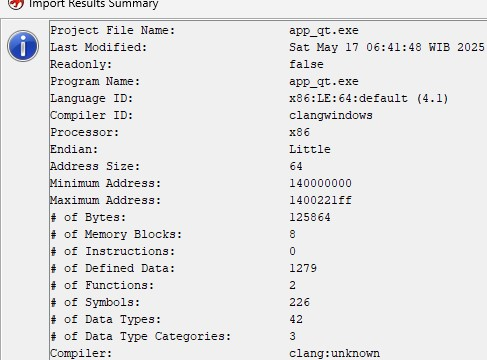
\includegraphics[width=0.9\linewidth]{../assets/pics/app_qt_summary_result.jpeg}
	\caption{Ghidra Analysis Summary for \texttt{app\_qt.exe} (Non-Virtualized).}
	\label{fig:ghidra_summary_qt_journal}
\end{figure}

\begin{figure}[!t]
	\centering
	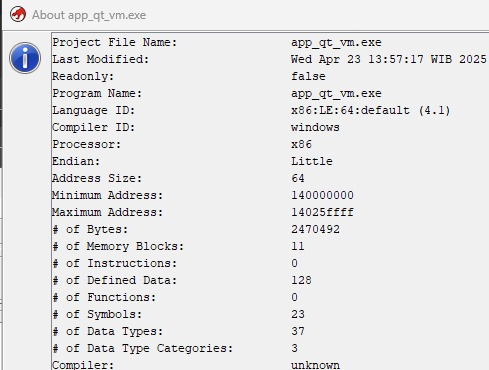
\includegraphics[width=0.9\linewidth]{../assets/pics/app_qt_vm_summary_result.jpeg}
	\caption{Ghidra Analysis Summary for \texttt{app\_qt\_vm.exe} (Virtualized, showing data for app\_qt\_vxm.exe structure).}
	\label{fig:ghidra_summary_qt_vm_journal}
\end{figure}

\subsubsection{Dynamic Analysis (x64dbg)}
\begin{itemize}
	\item \textbf{Non-Virtualized Binaries:} Dynamic analysis corroborated static findings. Setting breakpoints based on string references or near conditional jumps identified statically was effective. Stepping through the code clearly showed the comparison logic and the conditional jump execution. Runtime patching of the jump instruction in x64dbg successfully bypassed authentication (See example Listing \ref{lst:asm_dynamic_nonvirt_snippet} and context in Appendix Listing \ref{lst:asm_dynamic_nonvirt_full}).
	\item \textbf{Virtualized Binaries:} Dynamic analysis faced significant hurdles.
	      \begin{itemize}
		      \item \textit{String Searching Failure:} Searching for relevant strings in memory during runtime often failed, similar to static analysis.
		      \item \textit{Execution Flow Tracking Difficulty:} Stepping through the virtualized code sections was extremely difficult. The instruction pointer (RIP) often appeared to loop within small blocks or jump to seemingly random locations, consistent with execution being handled by the VM interpreter rather than direct native execution (See Listings \ref{lst:asm_dynamic_io_nonvirt_snippet} vs. \ref{lst:asm_dynamic_io_virt_snippet}, Appendix \ref{lst:asm_dynamic_io_comparison_full}). Standard debugging techniques like setting breakpoints based on expected native instructions became unreliable.
		      \item \textit{State Obfuscation:} Understanding the program's state (relevant variable values, comparison results) was hindered because the actual logic was executed within the VM's context, which was not directly visible or interpretable through the debugger's view of native registers and memory.
	      \end{itemize}
	      Dynamic bypass attempts by patching suspected native jump instructions (if any could be identified near the VM entry/exit) were unsuccessful, as the core logic resided within the VM's execution loop. The inability to trace execution flow coherently and the apparent looping or non-sequential jumps of the instruction pointer are characteristic of code execution being managed by an internal VM interpreter \cite{Sikorski2012}. While x64dbg, as a dynamic tool, can disassemble the native instructions of the VxLang VM itself, it does not directly reveal the original application logic, which has been translated into custom bytecode. The obfuscated state and hidden strings further complicated runtime understanding. Although debuggers can often resolve symbols for system DLLs loaded at runtime, internal application symbols within the virtualized segments remain obscured by VxLang, severely limiting the utility of dynamic analysis for understanding the protected code's semantics.
\end{itemize}

These results strongly indicate that VxLang's code virtualization effectively hinders both static and dynamic reverse engineering attempts using standard tools and techniques.

\subsubsection{Analysis of Lilith RAT}
Static and dynamic analysis were also performed on the Lilith RAT client (original vs. virtualized). Findings mirrored those from the authentication case studies:
\begin{itemize}
    \item \textbf{Non-Virtualized:} Analysis was feasible. Strings related to commands and functionality were identifiable. Control flow for network communication and command handling could be traced using Ghidra and x64dbg, allowing potential understanding of its mechanisms (e.g., keylogging, remote execution).
    \item \textbf{Virtualized:} Analysis difficulty increased significantly. Ghidra failed to properly disassemble virtualized sections, showing numerous '???' entries and obscuring the logic. Dynamic tracing in x64dbg was severely hampered by the VM execution, making it hard to follow command processing or data flow.
    \item \textbf{Functional Integrity:} Importantly, functional testing confirmed that the virtualized Lilith client (\texttt{Lilith\_Client\_vm.vxm.exe}) remained fully operational. In a two-machine local network setup (client IP: \texttt{192.168.1.15}, server IP: \texttt{192.168.1.235} on port \texttt{1337}), the virtualized client successfully connected to the unmodified Lilith server. The server operator was able to establish a remote command prompt session on the client machine (which was identified as \texttt{C:\textbackslash{}... \textbackslash{}bin\textbackslash{}Lilith\_Client\textbackslash{}Release>}), list directory contents, and successfully read a predefined test file (\texttt{password.txt}) containing the string \texttt{"THIS IS A SECRET"}. This demonstrated that VxLang's virtualization preserved core RAT functionalities such as network communication, remote command execution, and file system interaction, despite the significant code transformation.
\end{itemize}
This indicates VxLang's virtualization hinders analysis even for complex, potentially malicious software, without necessarily breaking its intended functionality.

\subsection{Performance and Size Overhead Results}

\subsubsection{Execution Time Overhead}
The performance impact was measured using QuickSort and AES benchmarks.

\begin{itemize}
	\item \textbf{QuickSort:} As shown in Table \ref{tab:quick_sort_performance_journal} and Fig. \ref{fig:quick_sort_performance_journal}, virtualization introduced substantial execution time overhead. The overhead increased with data size, ranging from approximately 27,300\% for 100 elements (0.01 ms to 2.74 ms) to about 15,150\% for 1,000,000 elements (218.32 ms to 33,292.91 ms). This indicates a significant constant overhead plus a scaling factor imposed by the VM's interpretation loop for the recursive sorting function.
	      \begin{table}[!t]
		      \centering
		      \caption{Quick Sort Execution Time Results (ms)}
		      \label{tab:quick_sort_performance_journal}
		      \resizebox{\columnwidth}{!}{%
			      \begin{tabular}{@{}lrrrr@{}}
				      \toprule
				      \multirow{2}{*}{\textbf{Array Size}} & \multicolumn{2}{c}{\textbf{Non-Virtualized}} & \multicolumn{2}{c}{\textbf{Virtualized}}                                        \\
				      \cmidrule(lr){2-3} \cmidrule(lr){4-5}
				                                           & \textbf{Avg Time}                            & \textbf{Std Dev}                         & \textbf{Avg Time} & \textbf{Std Dev} \\
				      \midrule
				      100                                  & 0.01                                         & 0.00                                     & 2.74              & 0.38             \\
				      1,000                                & 0.08                                         & 0.00                                     & 27.35             & 1.25             \\
				      5,000                                & 0.54                                         & 0.05                                     & 144.44            & 8.25             \\
				      10,000                               & 1.24                                         & 0.08                                     & 295.77            & 13.68            \\
				      50,000                               & 6.98                                         & 0.51                                     & 1,556.15          & 122.81           \\
				      100,000                              & 15.12                                        & 1.26                                     & 3,080.30          & 303.02           \\
				      500,000                              & 104.44                                       & 7.30                                     & 14,298.92         & 374.98           \\
				      1,000,000                            & 218.32                                       & 8.10                                     & 33,292.91         & 4,342.93         \\
				      \bottomrule
			      \end{tabular}
		      } % End resizebox
	      \end{table}

	      \begin{figure}[!t]
		      \centering
		      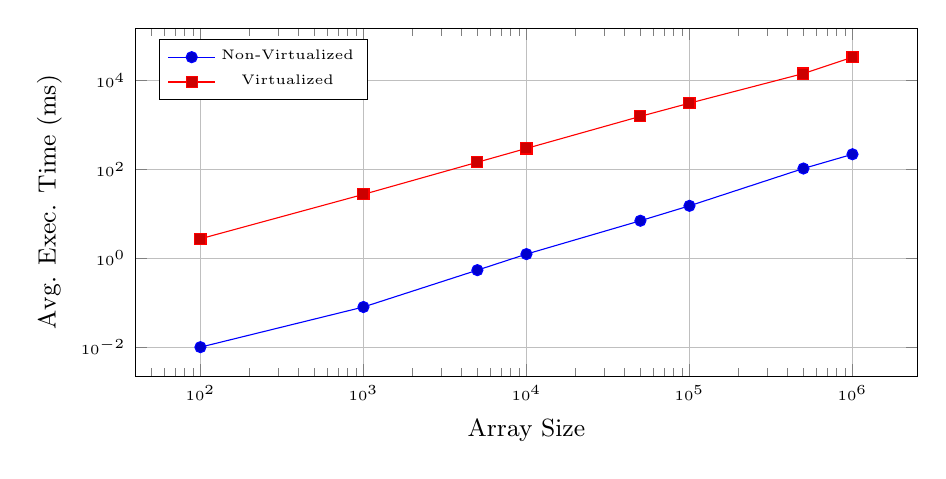
\begin{tikzpicture}
			      \begin{axis}[
					      width=0.95\columnwidth,
					      height=6cm,
					      xlabel={Array Size},
					      ylabel={Avg. Exec. Time (ms)},
					      xmode=log,
					      log basis x={10},
					      ymode=log,
					      log basis y={10},
					      legend pos=north west,
					      grid=major,
					      tick label style={font=\tiny},
					      label style={font=\small},
					      legend style={font=\tiny}
				      ]
				      \addplot coordinates {
						      (100, 0.01)
						      (1000, 0.08)
						      (5000, 0.54)
						      (10000, 1.24)
						      (50000, 6.98)
						      (100000, 15.12)
						      (500000, 104.44)
						      (1000000, 218.32)
					      };
				      \addlegendentry{Non-Virtualized};

				      \addplot coordinates {
						      (100, 2.74)
						      (1000, 27.35)
						      (5000, 144.44)
						      (10000, 295.77)
						      (50000, 1556.15)
						      (100000, 3080.30)
						      (500000, 14298.92)
						      (1000000, 33292.91)
					      };
				      \addlegendentry{Virtualized};
			      \end{axis}
		      \end{tikzpicture}
		      \caption{Quick Sort Execution Time Comparison (Log-Log Scale).}
		      \label{fig:quick_sort_performance_journal}
	      \end{figure}


	\item \textbf{AES Encryption:} Table \ref{tab:aes_performance_journal} shows that the total time for encrypting 976MB of data increased by approximately 396.7\% (1878.52 ms to 9330.73 ms), and decryption time increased by about 562.9\% (1304.75 ms to 8649.74 ms). Consequently, the combined throughput dropped dramatically from 634.16 MB/s to 108.78 MB/s (an 82.8\% reduction). This confirms a significant overhead for cryptographic operations.
	      \begin{table}[!t]
		      \centering
		      \caption{AES-256-CBC Performance Results (976MB Data)}
		      \label{tab:aes_performance_journal}
		      \resizebox{\columnwidth}{!}{%
			      \begin{tabular}{@{}lrr@{}}
				      \toprule
				      \textbf{Metric}              & \textbf{Non-Virtualized} & \textbf{Virtualized} \\
				      \midrule
				      Total Encryption Time (ms)   & 1,878.52                 & 9,330.73             \\
				      Total Decryption Time (ms)   & 1,304.75                 & 8,649.74             \\
				      Avg. Encrypt Time/Block (ms) & 0.00188                  & 0.00933              \\
				      Avg. Decrypt Time/Block (ms) & 0.00130                  & 0.00865              \\
				      Encrypt Throughput (MB/s)    & 519.86                   & 104.66               \\
				      Decrypt Throughput (MB/s)    & 748.46                   & 112.90               \\
				      Combined Throughput (MB/s)   & 634.16                   & 108.78               \\
				      \bottomrule
			      \end{tabular}
		      } % End resizebox
	      \end{table}

\end{itemize}

\subsubsection{File Size Overhead}
Table \ref{tab:file_size_journal} shows a consistent increase in executable file size after virtualization. For smaller console/benchmark programs (\texttt{quick\_sort}, \texttt{encryption}, \texttt{console}, \texttt{Lilith\_Client}), the size increased by over 15-18 times (from ~80-110 KB to ~1.5-1.6 MB). For larger GUI applications (\texttt{app\_imgui} from 1,675 KB to 2,330 KB; \texttt{app\_qt} from 122 KB to 1,578 KB) and the benchmark with embedded data (\texttt{size} from 97,771 KB to 112,324 KB), the relative increase was smaller but still significant. This overhead is primarily attributed to the inclusion of the VxLang VM runtime and the bytecode representation of the original code.
\begin{table}[H]
	\centering
	\caption{Executable File Size Comparison (KB)}
	\label{tab:file_size_journal}
	\resizebox{\columnwidth}{!}{
		\begin{tabular}{@{}lrr@{}}
			\toprule
			\textbf{Program}  & \textbf{Non-Virtualized (KB)} & \textbf{Virtualized (KB)} \\
			\midrule
			quick\_sort       & 98                            & 1,537                     \\
			encryption        & 110                           & 1,507                     \\
			size              & 97,771                        & 112,324                   \\
			console           & 92                            & 1,577                     \\
			console\_cloud    & 281                           & 1,695                     \\
			app\_imgui        & 1,675                         & 2,330                     \\
			app\_imgui\_cloud & 1,860                         & 2,418                     \\
			app\_qt           & 122                           & 1,578                     \\
			app\_qt\_cloud    & 315                           & 1,671                     \\
			Lilith\_Client    & 84                            & 1,554                     \\
			\bottomrule
		\end{tabular}
	}
\end{table}

\subsection{VirusTotal Detection Analysis}
To assess the impact of VxLang virtualization on automated malware detection, both the original and virtualized Lilith RAT client executables  were submitted to VirusTotal.

\begin{itemize}
	\item \textbf{Non-Virtualized Lilith:} Detected by \textbf{22 out of 72} engines. Analysis revealed specific threat labels like "trojan.lilithrat/keylogger" and family labels including "lilithrat" and "keylogger". Detections often included specific names like "Backdoor:Win64/LilithRat.GA!MTB" or "Trojan[Backdoor]/Win64.LilithRAT".
	\item \textbf{Virtualized Lilith:} Detected by \textbf{18 out of 72} engines, showing a decrease in detection rate. The popular threat label became a generic "trojan", and specific family labels disappeared. Detection signatures shifted towards generic malware, heuristic-based flags, AI/ML detections, or packed/protected software warnings (e.g., "Trojan:Win32/Wacatac.C!ml", "Static AI - Suspicious PE", "ML.Attribute.HighConfidence", "RiskWare[Packed]/Win32.VMProtect.a").
\end{itemize}
These results suggest that VxLang virtualization effectively obfuscates static signatures used by many traditional antivirus engines, forcing reliance on less specific heuristic or AI-based methods, and potentially evading detection by some vendors altogether.

\subsection{Discussion}
The experimental results clearly demonstrate the core trade-off inherent in using VxLang's code virtualization.

\textbf{Security Enhancement and Detection Evasion:} VxLang provides a substantial barrier against common reverse engineering techniques. The transformation into interpreted bytecode neutralizes standard static analysis tools like Ghidra, which rely on recognizable native instruction patterns \cite{Eilam2011, Ko2007}, and significantly complicates dynamic analysis with tools like x64dbg, as the underlying logic is executed by an opaque VM \cite{Sikorski2012}. This aligns with the established understanding that VM-based obfuscation fundamentally alters the code structure beyond the interpretation capabilities of standard disassemblers \cite{Ore06, Sal18}. Furthermore, the VirusTotal analysis indicates that this obfuscation extends to automated malware detection; VxLang effectively hinders signature-based detection, reduces overall detection rates, and forces AV engines towards more generic or heuristic approaches. This capability to evade specific detection signatures adds another layer to its protective potential, aligning with the expected benefits of advanced obfuscation \cite{Ore06, Sal18, Rou13}.

\textbf{Performance Cost:} The security and evasion benefits come at a steep price in terms of performance. The interpretation overhead significantly slows down virtualized code, especially for computationally intensive tasks (QuickSort overhead of ~15,000\% for 1M elements; AES throughput reduction of ~83\%), potentially rendering indiscriminate application impractical due to severe speed degradation.

\textbf{Size Increase:} The considerable increase in file size (e.g., 15-18x for small applications), mainly due to the embedded VM runtime, is another factor, particularly relevant for smaller applications or distribution constraints.

\textbf{Practical Implications:} VxLang appears potent for protecting highly sensitive code where security and potentially detection evasion are paramount, and the performance impact on those specific segments is acceptable (e.g., anti-tamper, licensing, core IP). The Lilith case shows it can protect complex logic without breaking it. However, the severe performance cost necessitates a strategic, selective application, targeting only critical sections. The VirusTotal results also imply that while detection is hindered, it's not eliminated, especially by heuristic/AI methods or tools flagging the protection layer itself. The choice between hardcoded and cloud-based authentication showed that protecting client-side logic handling the result of validation remains crucial, reinforcing the need for techniques like virtualization on critical checks, regardless of where primary authentication occurs.

\section{Conclusion} \label{sec:conclusion}
This paper investigated the effectiveness of code virtualization using the VxLang framework as a technique to mitigate software reverse engineering. The process involved marking code with SDK macros, compiling intermediate executables (\texttt{*\_vm.exe}), and processing them directly via the \texttt{vxlang.exe} command-line tool to generate final virtualized binaries (\texttt{*\_vxm.exe}). Through experimental analysis involving static (Ghidra) and dynamic (x64dbg) examination of authentication applications and performance benchmarking (QuickSort, AES), we draw the following conclusions:

VxLang's code virtualization significantly enhances software security by substantially increasing the difficulty of reverse engineering. The transformation into custom bytecode rendered standard static analysis tools ineffective at interpreting program logic and control flow within virtualized sections. Dynamically, while x64dbg could observe the native instructions of the VxLang Virtual Machine (VM) itself during runtime, the core application logic remained effectively obscured. Critical strings targeted by virtualization were not discoverable via standard debugger searches, and the abstraction of the application's decision-making processes into the VM's bytecode execution made direct runtime manipulation (e.g., patching conditional jumps for authentication bypass) unfeasible. Attempts to bypass authentication logic, which were trivial in non-virtualized versions, were successfully thwarted in the virtualized binaries using the employed static and dynamic analysis techniques. \textbf{However, the application of these protective measures required careful, iterative placement of virtualization macros, as improper application, particularly in complex code sections involving I/O or intricate control flows, was found to potentially disrupt software functionality, as observed with the Lilith RAT case study.}

Furthermore, analysis of a virtualized RAT (Lilith) showed maintained functionality alongside reduced detection rates and a shift from specific signatures to generic flags on VirusTotal, demonstrating VxLang's capability to also evade traditional antivirus detection mechanisms.

However, this robust security comes with significant drawbacks. We observed substantial performance overhead, with execution times for computational tasks increasing dramatically (by factors ranging from hundreds to tens of thousands) after virtualization. Furthermore, the inclusion of the VxLang VM runtime and bytecode resulted in a considerable increase in executable file size, particularly impactful for smaller applications.

The findings highlight a clear trade-off: VxLang provides strong protection against reverse engineering at the cost of significant performance degradation and increased file size. Therefore, its practical application likely requires a selective approach, targeting only the most critical and sensitive code sections where the security benefits outweigh the performance impact.

Future work could involve exploring more advanced reverse engineering techniques specifically targeting VM-based protections to further assess VxLang's resilience. Investigating the impact of different VxLang configuration options on the security-performance balance would also be valuable. \textbf{Further research into the specific code constructs or patterns that interact poorly with VxLang's virtualization process could yield guidelines for more robust and reliable application of such protection mechanisms.} Comparative studies with other commercial or open-source virtualization solutions could provide a broader perspective. Investigating the interaction between VxLang and various antivirus detection techniques (signature-based, heuristic, AI/ML, behavioral) would also yield valuable insights into its detection evasion capabilities and limitations.


% --- Optional Sections ---
% \appendices % If you have appendices
% \section{Proof of the Zonklar Equation}
% Appendix one text goes here.

% \section*{Acknowledgment} % Use section* for unsnumbered sections
% % use section* for acknowledgment
\section*{Acknowledgment}


The authors would like to thank...
 % Input the acknowledgment content


% --- References ---
% Print the bibliography using BibLaTeX
\printbibliography

% --- Optional Biographies ---
% \newpage % If biographies need to start on a new page

% \begin{IEEEbiography}[{\includegraphics[width=1in,height=1.25in,clip,keepaspectratio]{path/to/your/photo.png}}]{Seno Pamungkas Rahman}
% received the B.Eng. degree in Computer Engineering from the Universitas Indonesia, Depok, Indonesia, in 2025. His research interests include software security, reverse engineering, code obfuscation, and system programming.
% \end{IEEEbiography}

% \begin{IEEEbiographynophoto}{Dr. Ruki Harwahyu}
% Biography text here. Include degrees, affiliations, research interests, memberships (e.g., Member, IEEE).
% \end{IEEEbiographynophoto}

% You can push biographies down or up by placing
% a \vfill before or after them. The appropriate
% use of \vfill depends on what kind of text is
% on the last page and whether or not the columns
% are being equalized.

%\vfill

% Can be used to pull up biographies so that the bottom of the last one
% is flush with the other column.
%\enlargethispage{-5in}

\end{document}
